\section{Python} \label{pythonstructure}
The Python part of the project is separated into multiple modules.
The intention of a modular structure is to allow for a system that can be easily modified, based on the specific context.

For the project, the following modules are used:
\begin{itemize}
	\item Object Localization Algorithm
	\item Output / Communication
	\item Input / Webcam
	\item Calibration
\end{itemize}

\autoref{fig:pythonClasses} shows the dependencies of each of the actual packages, and how each module is split up, into multiple packages or files.

\begin{figure}[H]
	\centering
	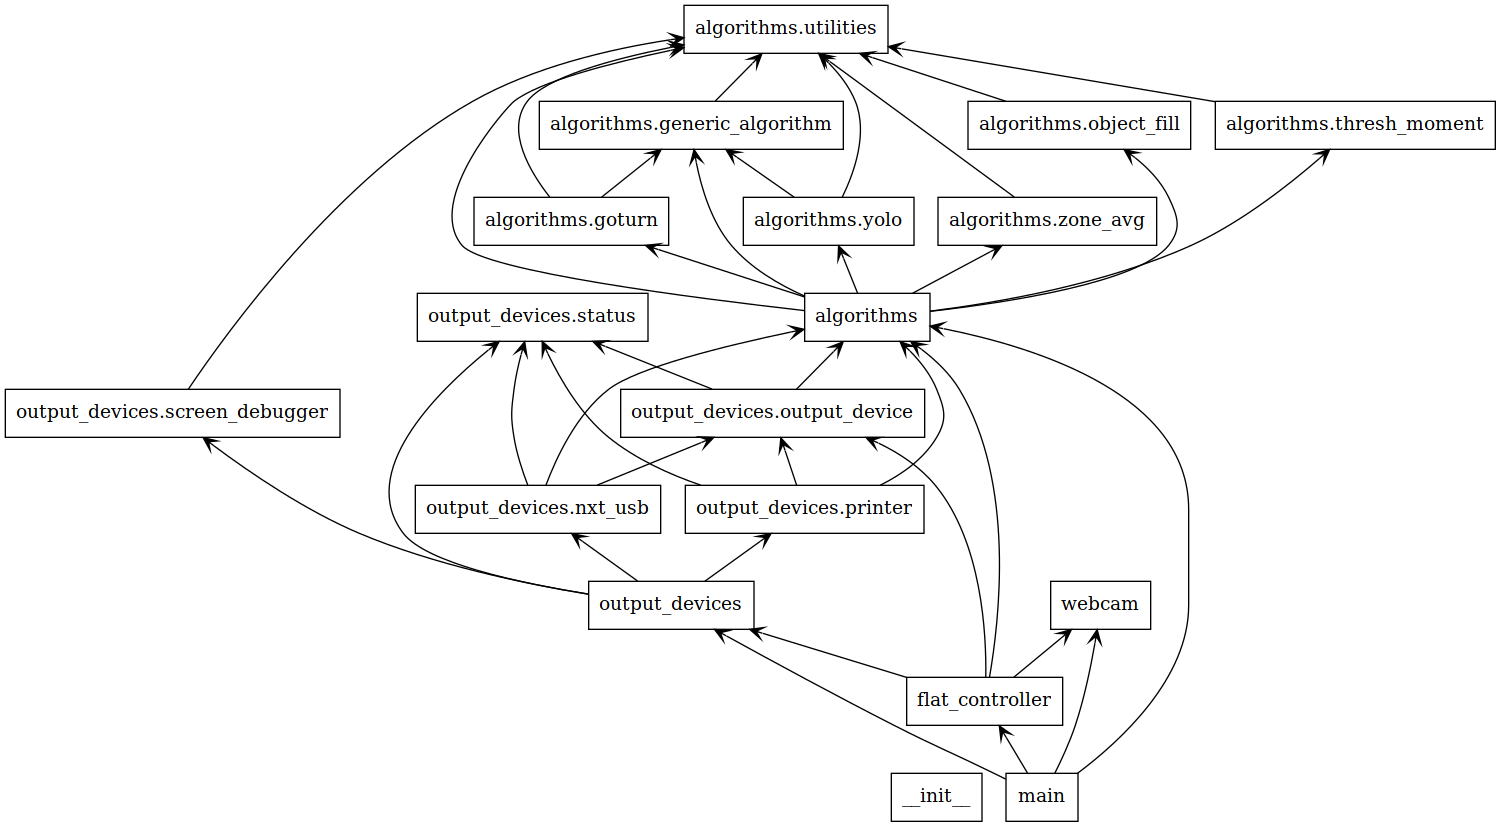
\includegraphics[width=\textwidth]{5.Solution/images/python_packages.png}
	\caption{The dependencies of the packages of the project{.} Image generated with pyreverse\cite{pyreverse}}
	\label{fig:pythonClasses}
\end{figure}


The project also contains functions for calibration, as seen on \autoref{fig:pythonClasses}, which will be covered in \autoref{sec:calibration}.

\subsection{Main.py}
The entry point for the python program is \texttt{main.py}.
The arguments for \texttt{main.py}  are shown in \autoref{lst:MainHelp}.
\begin{lstlisting}[label={lst:MainHelp},caption={The help message of the commandline interface}]
$ python3 main.py --help
usage: main.py [-h] [-a [name]] [-n [no_usb]]

Run the object detection part of the F.L.A.T system

optional arguments:
-h, --help            show this help message and exit
-a [name], --algorithm [name]
Choose which algorithm to run [ZONE_AVG, OBJ_FILL,
THRESH_MOMENT] default='thresh_moment'
-n [no_usb], --no-usb [no_usb]
Whether to disable USB connection with the NXT.
default=False
\end{lstlisting}

The main objective of \texttt{main.py} is to determine which arguments to pass onto the \texttt{FlatController}.

\subsection{FlatController}\label{flatcontrollerimplementation}
The \texttt{FlatController} class manages the different modules of the Python part of the project and ties the Python part of the solution together
The signature of the \texttt{FlatController} is shown in \autoref{lst:FlatControllerInit}.

\begin{lstlisting}[language=Python,label={lst:FlatControllerInit},caption={Initialization method of the \texttt{FlatController} class}]
	def __init__(self,
		algorithm: Callable[[np.ndarray], Optional[Vector]],
		output_device: OutputDevice,
		input_device: VideoController,
		calibration_algorithm: Union[Callable[[OutputDevice], None], None] = None,
		debug=True
		) -> None:
\end{lstlisting}

The order of the parameters are not an indication of their relevance, but is rather based on the requirement of Python itself, as Python requires parameters with default parameters to be first in the signature of the methods.

The method takes a function, \texttt{algorithm} with an array as input and a vector as output.
The function is a specification of the specific algorithm to use for image recognition.
The array is the array of pixels in a given frame, while the vector is the center of the found object in the image.

The \texttt{output\_device} parameter, specifies how to output the location data.
This can be direct transmission of data to the NXT or it can use a video feed, which is used for debugging and getting the video output of the what the \texttt{F.L.A.T}'s camera.

The \texttt{input\_device} parameter specifies which device the video feed should be received from.
This is primarily a live video feed taken from the \texttt{F.L.A.T}'s camera, but can also be video file.
The video file option was primarily used for testing.

The \texttt{calibration\_algorithm} is relevant when connected to an NXT and calibration is needed.
The calibration algorithm will send a request to the NXT, asking it to begin calibrating, after which the \texttt{calibration\_algorithm} will wait for the arrival of the calibration data from the NXT.

The \texttt{calibration\_algorithm} handles this information depending on implementation, the default implementation is simply storing this data for later usage.

Finally, the \texttt{debug} parameter specifies whether the program is in debug mode.
When in debug mode, various relevant information is posted to the screen, along with a live video feed.
The information includes the current tick count, the current frames per second and the current location found.

